\appendix

\section{Proof of Example~1}
Consider the function $f:\mathbb{R}\rightarrow\mathbb{R}$ defined by
\begin{equation}
	f(x)=w_2^T \sigma(w_1 x + b_1) + b_2,
\end{equation}
where $\sigma$ is the ReLU activation function, $w_1,w_2,b_1\in\mathbb{R}^n$, and $b_2\in\mathbb{R}$. Our goal is to characterize the slopes of this function at $+\infty$ and $-\infty$, assuming that $\|w_1\|\leq 1$ and $\|w_2\|\leq 1$.

Writing the function explicitly in terms of the entries of the parameter vectors, we obtain
\begin{equation}
f(x)=\sum_{i=1}^n (w_2)_i \cdot\max\left\{(w_1)_i\, x + (b_1)_i,0\right\} + b_2.
\end{equation}
Therefore, 
\begin{equation}
f'(x)=\sum_{i\in\mathcal{I}_x}(w_1)_i (w_2)_i,
\end{equation}
where
\begin{equation}
\mathcal{I}_x=\{i:(w_1)_i\,x+(b_1)_i>0\}.
\end{equation}
Now, note that 
\begin{align}
\mathcal{I}_\infty=\{i:(w_1)_i>0\}, \qquad
\mathcal{I}_{-\infty}=\{i:(w_1)_i<0\}.
\end{align}
We thus have that
\begin{align}
|f'(-\infty) + f'(\infty)| &= \left|\sum_{i\in\mathcal{I}_{-\infty}}(w_1)_i (w_2)_i + \sum_{i\in\mathcal{I}_{\infty}}(w_1)_i (w_2)_i\right| \nonumber\\
&= \left|\sum_{i=1}^n(w_1)_i (w_2)_i\right| \nonumber\\
&\leq  \|w_1\|\, \|w_2\| \nonumber\\
&\leq 1,
\end{align}
where in the second line we added to the sum all indices $i$ for which $(w_1)_i=0$ (the sum over these indices gives zero), in the third line we used Parseval's inequality, and in the last line we used the fact that $\|w_1\|\leq 1$ and $\|w_2\|\leq 1$.


\section{Proof of Lemma~1}
For a single-input-single-output cyclic convolution operation, $y=h*x$, it is well known that the top singular value is $\|\mathcal{F}\{h\}\|_\infty$, the maximal absolute value of the discrete Fourier transform of $h$ (after zero-padding it to the length of $x$). Now, for a multiple-input-multiple-output convlution $W$, we have
\begin{align}
\|W\|_{0,\infty} &= \sup_{\|\boldsymbol{x}\|_0 \leq 1\atop\|\boldsymbol{x}\|_\infty \leq 1} \|W\boldsymbol{x}\|_\infty \nonumber\\
&= \sup_{\|\boldsymbol{x}\|_0 \leq 1\atop\|\boldsymbol{x}\|_\infty \leq 1} \max_{i}\Big\|\sum_j w_{i,j}*x_j\Big\| \nonumber\\
%& \leq  \sup_{\|\boldsymbol{x}\|_0 \leq 1\atop\|\boldsymbol{x}\|_\infty \leq 1} \max_{i}\sum_j\| w_{i,j}*x_j\| \nonumber\\
& =  \sup_{\|\boldsymbol{x}\|_\infty \leq 1} \max_j \max_{i}\| w_{i,j}*x_j\| \nonumber\\
& =  \max_j \max_{i} \sup_{\|x_j\| \leq 1}\| w_{i,j}*x_j\| \nonumber\\
& =  \max_j \max_{i} \|\mathcal{F}\{w_{i,j}\}\|_\infty,
\end{align}
where in the third line we used the fact that when $\|\boldsymbol{x}\|_0 \leq 1$, the sum contains only one nonzero element, and in the last line we used the top singular value of a single-input-single-output convolution.

\begin{figure*}[h]
\begin{center}
%\vspace{-3cm}
\begin{tabular}{ p{8cm} c }  
\vspace{-1.75cm}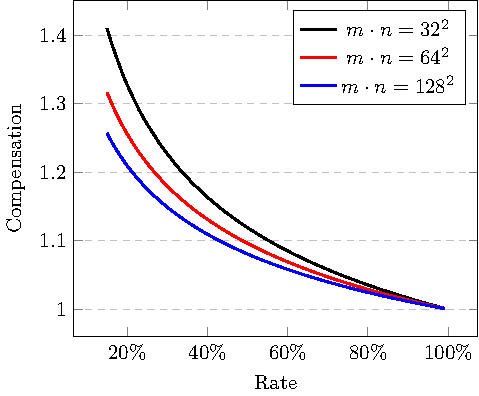
\includegraphics[width=0.4\textwidth]{./compensation.pdf}
&
\renewcommand{\arraystretch}{2}
\begin{tabular}{ll|l|l|l|l|}
        
\multicolumn{2}{c}{}&   \multicolumn{4}{c}{Compensation}\\
\multicolumn{2}{c}{}&\multicolumn{4}{c}{
              {\rotatebox[origin=c]{0}{    1.0    }
            } {\rotatebox[origin=c]{0}{    1.1    }
            } {\rotatebox[origin=c]{0}{    1.2    }
            } {\rotatebox[origin=c]{0}{    1.3    }
        }}\\
\cline{3-6}
\multirow{3}{*}{{\rotatebox[origin=c]{90}{Rate}
}} & 
100\% & 73.8 & \textbf{65.8} & 78.8 & 69.6  \\ \cline{3-6}
&   50\%  & 76.6 & 73.6 & \textbf{72.4} & 79.3 \\ \cline{3-6}
&   25\%  & 74.3 & 74.7 & 75.2 & \textbf{67.8} \\ \cline{3-6}
\end{tabular}\\
& \\
\end{tabular}
\caption{\textbf{Compensation factor.} The left pane depicts the theoretical compensation factor $g$ for varied filter sizes, as a function of the percentage of filters $r$ used to compute the normalization constant. The table on the right details the Fr\'echet Inception distance (FID) attained in Cityscapes label-to-image translation, for different ratios and compensation factors. As can be seen, the optimal compensation factor indeed increases as the ratio of filters decreases.}
\label{fig:study_compensation}
\end{center}
\end{figure*} 

\begin{algorithm*}
\caption{SGD with sparsity aware normalization (SAN))}\label{alg:san}
\begin{algorithmic}[1]
\For {each layer, $\ell = 1, \dots, n$}

\State Calculate $\sigma$ from a random subset of filters $\{\tilde{w}^\ell_{i,j}\} \subset \{w^\ell_{i,j}\}$,
\begin{align*}
\sigma = \max_{i,j}\|\mathcal{F}\{\tilde{w}_{i,j}\}\|_\infty.
\end{align*}
\State Normalize $W^\ell$ using a compensation factor $g$,
\begin{align*}
W^\ell \leftarrow W^\ell / (g \cdot \sigma) .
\end{align*}
\State Update $W^\ell$ using a mini-batch of $M$ samples with a learning rate of $\alpha$, as
\begin{equation*}
W^\ell \leftarrow W^\ell - \alpha \tfrac{1}{M}\sum_{i=1}^{M}\nabla_{W^\ell}\mathcal{L}(x_i,y_i), 
\end{equation*}
where $\mathcal{L}(x_i,y_i)$ is the critic loss for input $x_i$ and label $y_i$.

\EndFor


\end{algorithmic}
\end{algorithm*}

\section{The Compensation Factor}
Next, we study the compensation factor $g$ that has to be used when computing our normalization constant based on only a (random) subset of the filters. Figure~\ref{fig:hist_ffts} depicts the histogram of values $\{ \|\mathcal{F}\{w_{i,j}\}\|_\infty\}$ for the last layer of the standard critic network used in the paper. This layer has  $m=256$ input channels and $n=512$ output channels, so that the histogram is over  $256\times 512\approx 130,000$ values. As can be seen, the decay of the histogram is roughly exponential. This suggests that the values $\{ \|\mathcal{F}\{w_{i,j}\}\|_\infty\}$ can be regarded as realizations of independent random variables $\{X_j\}_{j=1}^{m\cdot n}$ distributed $\text{exp}(\lambda)$, for some $\lambda>0$. Now, assuming we compute the maximum over only $k<m\cdot n$ values, we would like to know how much smaller the result would be on average. Namely, we would like to compare $\E[\max \{X_j\}_{j=1}^k]$ with $\E[\max \{X_j\}_{j=1}^{m\cdot n}]$.

In \cite{renyi1953theory}, Alfr\'ed R\'enyi showed that the $i$th order statistics of $k$ iid samples from an exponential distribution is given by
\begin{equation}
X_{(i)} \overset{d}{=}  \frac{1}{\lambda} \left(\sum_{j=1}^{i} \frac{Z_j}{k-j+1}\right),
\label{eq:order_distribution}
\end{equation}
where $\overset{d}{=}$ denotes equality in distribution and the $Z_j$ are iid standard exponential random variables (with $\lambda=1$). Thus, focusing on the maximum, which corresponds to $i=k$, and taking the expectation of the expression, we obtain
\begin{equation}
\E \left[\max\{X_j\}_{j=1}^k\right] = \frac{1}{\lambda} \left(\sum_{j=1}^{n} \frac{1}{n-j+1}\right),
\label{eq:order_maxium}
\end{equation}
Therefore, when taking a ratio of $r$ of the filters (so that $k=\round{m \cdot n \cdot r}$, the compensation factor should be taken to be
\begin{equation}
g=\frac{\E \left[\max\{X_j\}_{j=1}^{m\cdot n}\right]}{\E \left[\max\{X_j\}_{j=1}^{\round{m \cdot n \cdot r}}\right]}=\frac{\sum_{j=1}^{m\cdot n} \frac{1}{m\cdot n-j+1}}{\sum_{j=1}^{\round{m \cdot n \cdot r}} \frac{1}{\round{m \cdot n \cdot r}-j+1}}.
\label{eq:compensation_factor}
\end{equation}

\begin{figure}[h!]
\centering
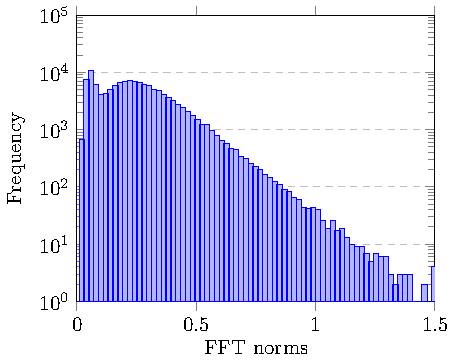
\includegraphics[width=0.8\columnwidth]{./standard_l6.pdf}
\caption{\textbf{Exponential decay}. The histogram of values $\{ \|\mathcal{F}\{w_{i,j}\}\|_\infty\}$ for the last layer of the standard critic network used in the paper.}
\label{fig:hist_ffts}
%\vspace{-0.5cm}
\end{figure}

Interestingly, this value varies quite slowly with $r$ for large $m$ and $n$. This can be seen in Fig.~\ref{fig:study_compensation} (left), where we depict the theoretical optimal value $g$ of \eqref{eq:compensation_factor} for varied filters sizes. For example, $g$ typically does not exceed $1.3$ even for ratios as low as $25\%$.


To verify Eq.~\eqref{eq:compensation_factor}, we also conduct an experiment on the task of Cityscapes label-to-image translation task. For this objective, we adopt the SPADE \cite{spade} framework with narrower generator and discriminator networks as a baseline, apply SAN in the discriminator and train several models with different ratios $r$ and compensation factors $g$. In Fig.~\ref{fig:study_compensation} (right), we show the Fr\'echet Inception distances (FID) attained for each model. The best result is attained with a rate and compensation of $100\%$ and $1.1$, respectively. Furthermore, the practical optimal compensation factor roughly agrees with the theoretical one for rates lower than $100\%$.

\section{The Sparsity Aware Normalization Algorithm}

Algorithm \ref{alg:san} describes the SAN algorithm update of the critic within an SGD step. In models for large images, we compute the normalization constant over a random subset of the filters as is determined by Eq.~\eqref{eq:compensation_factor}.


\section{Ablation Study}

\begin{figure}[t]
\centering

\includegraphics[width=0.75\columnwidth]{./training.pdf}
\caption{\textbf{Convergence}. Inception score on CIFAR-10 during training with three WGANs different methods.}
\label{fig:convergence}
\end{figure}


In this section, we explore and evaluate our sparsity aware normalization on a series of experiments. We focus on image generation for CIFAR-10 with the standard CNN architecture, and compare the inception score (IS) of our SAN-GAN to those of spectral normalization (SN-GAN) \cite{spectral} and an un-normalized GAN variant (Vanilla). In all the experiments, the number of updates for the generator is set to $80$K, and all methods are initialized with the same draw of random weights


To explore how the usage of our normalization impacts the optimization of WGANs, we measure the inception score (IS) of the three methods during training. As shown in Fig.~\ref{fig:convergence}, our method exhibits a faster and steadier convergence.


We continue by preforming an ablation study on the looseness of the normalization. As loosening the bound in our $\|\boldsymbol{\cdot}\|_0$ constraint is computationally impractical, we focus only on loosening the $\|\boldsymbol{\cdot}\|_\infty$ bound, which boils down to multiplying the normalization constant by some correction. Therefore, in practice, this implies using a different compensation factor $g$. In Fig.~\ref{fig:looseness_norm}, we vary the magnitude of the norm constraint between $0.5$ and $1.5$. Interestingly, we obtained the best results with a value of $1.1$, a small improvement over the results with $1.0$, which is proposed in the paper. This suggests that our approach, with a bound of $1.0$ does actually predict a rather good normalization
constant.


To characterize the dependence of our sparsity aware normalization on the training configuration, we inspect all three methods under six hyper-parameter settings (A-F) corresponding to different learning rates $\alpha$,  different first and second order momentum parameters $(\beta_1, \beta_2)$ for the Adam optimizer, and different numbers of critic updates for each generator update, $n_\text{dis}$. As can be seen in Fig. \ref{tab:study_confs}, our method outperforms spectral normalization in all settings except for E. This is true even with a high learning rate, where spectral normalization fails (set A). These results suggest that our method is more robust than the competing methods to perturbations in the training settings.

\begin{figure}[t]
\centering
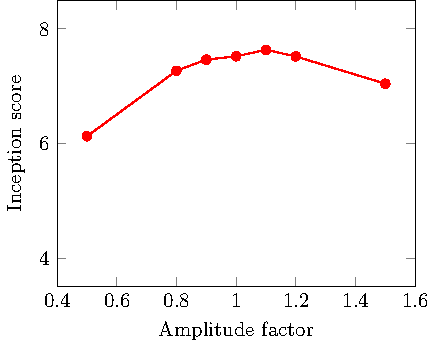
\includegraphics[width=0.775\columnwidth]{./amp.pdf}
\caption{\textbf{Looseness of normalization}. Inception score on CIFAR-10 for different $\ell_\infty$ norm constraints.}
\label{fig:looseness_norm}
\end{figure}


\begin{figure*}[h]
	\begin{center}
		\vspace{-3cm}
		\begin{tabular}{ p{7cm} c }  
			\vspace{0cm}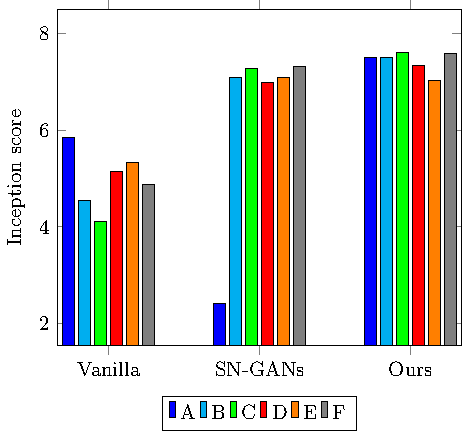
\includegraphics[width=0.33\textwidth]{./configurations.pdf}
			&
			\begin{tabular}{ L{1.2cm} C{1cm} C{0.6cm} C{0.6cm} C{0.6cm} }
				\\ \\ \\ \\ \\ \\ \\ \\ \\
				Setting & $\alpha$ & $\beta_1$ & $\beta_2$ & $n_{\text{dis}}$ \\ \hline
				A & $0.0005$ & $0.5$ & $0.9$ & $1$ \\
				B & $0.0002$ & $0.5$ & $0.9$ & $1$ \\
				C & $0.0002$ & $0$ & $0.9$ & $1$ \\
				D & $0.0005$ & $0$ & $0.9$ & $1$ \\
				E & $0.0002$ & $0.5$ & $0.9$ & $2$ \\
				F & $0.0005$ & $0$ & $0.9$ & $2$ \\
			\end{tabular}\\
			& \\
		\end{tabular}
		\caption{\textbf{Resistance to training hyper-parameters.} Inception scores on CIFAR-10 with different methods and training hyper-parameters.}
		\label{tab:study_confs}
	\end{center}
\end{figure*}

\begin{figure*}[h]
	\begin{center}
		\vspace{-3cm}
		\begin{tabular}{ p{10cm} c }  
			\vspace{0cm}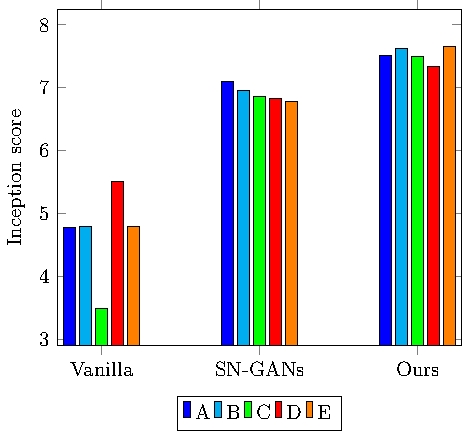
\includegraphics[width=0.33\textwidth]{./seed.pdf}
			&
			\begin{tabular}{ L{1.2cm} C{1.2cm} }
				\\ \\ \\ \\ \\ \\ \\ \\ \\
				Setting & \# seed \\ \hline
				A & $5354$ \\
				B & $9017$ \\
				C & $11224$ \\
				D & $5577$ \\
				E & $61$ \\
			\end{tabular}\\
			& \\
		\end{tabular}
		\caption{\textbf{Robustness to weight initialization.} Inception scores on CIFAR-10 with different methods and initial weight sets.}
		\label{tab:study_seed}
	\end{center}
\end{figure*}

To see how sensitive the results are to the particular weight initialization, in Fig.~\ref{tab:study_seed} we show the inception scores of each method with set B for several different seeds of the random number generator. As can be seen, our method consistently outperforms the competitors, indicating that it is more robust to the specific draw of the weights at initialization. 


\section{Running Time}
On CIFAR-10, SAN-GANs is slightly slower than running with no normalization ($\sim +15\%$ in computation time), is similar to spectral normalization ($\sim +2\%$ in computation time), but significantly faster than WGAN-GP ($\sim -17\%$ in computation time). Specifically, on our system, for one critic iteration update for the ``standard'' network (Table~\ref{tab:arch_gen_standard}), the average computation times are:
\begin{itemize}

\vspace{-0.05cm}

\item Vanilla: $35.74ms$
\vspace{-0.05cm}

\item WGAN-GP: $50.02ms$
\vspace{-0.05cm}

\item Spectral-Norm: $40.51ms$
\vspace{-0.05cm}

\item Ours: $41.45ms$
%\vspace{-0.05cm}

\end{itemize}

It is important to note, however, the $15\%$ overhead for one update typically does not translate to a $15\%$ overhead in the total training time. This is because, as discussed above, we do not have to use our normalization every update step and we can compute the normalization constant over only a random subset of filters. 

\section{Image-to-Image Translation}

\begin{table*}[t]
%\tiny
\begin{center}
\begin{tabular}{c c c c c c c }
%\begin{tabular}{p{0.5cm} p{0.5cm} p{0.5cm} p{0.5cm} p{0.5cm} c c}
\centering
Black & Blond & Brown & Female & Male & StarGAN & SAN-StarGAN \\ \hline
\ding{51} & \ding{55} & \ding{55} & \ding{51} & \ding{55} & 85.10 & \textbf{71.41}\\
\ding{51} & \ding{55} & \ding{55} & \ding{55} & \ding{51} & 88.72 &  \textbf{81.01}\\
			
\ding{55} & \ding{51} & \ding{55} & \ding{51} & \ding{55} & 189.65 & \textbf{184.82}\\
\ding{55} & \ding{51} & \ding{55} & \ding{55} & \ding{51} & 117.06 & \textbf{100.51}\\
			
\ding{55} & \ding{55} & \ding{51} & \ding{51} & \ding{55} & 101.33 & \textbf{87.91}\\
\ding{55} & \ding{55} & \ding{51} & \ding{55} & \ding{51} & 87.15 &  \textbf{76.32}\\
			
\end{tabular}
\end{center}
\caption{Quantitative comparison on the task of gender translation. The left 5 columns describe the source domain. The target domain corresponds to the same hair color, but the opposite gender. The Fr\'echet inception distance (FID) measures the discrepancy between the distributions of real and generated images (lower is better).}
\label{tab:image2image}
\end{table*}
\addtolength{\tabcolsep}{-3pt} 

Here, we provide additional image-to-image translation results for our method. Specifically, we use the CelebA dataset \cite{celeba} and focus on the task of modifying a particular attribute of an input image, like gender or hair color, to have some desired value, like male/female or black/blond/brown. We adopt StarGAN scheme \cite{stargan} as a baseline framework, and enhance its results by incorporating our normalization. As in \cite{stargan}, we take the generator to comprise two convolution layers with stride 2 (for downsampling), followed by six residual blocks, and two transposed convolution layers with stride 2 (for upsampling). For the critic, we use six convolution layers with circular padding, but reduce the kernel size from $4 \times 4$ to $3 \times 3$, so that the number of parameters in our model is only $25$M (in contrast to the $44$M of \cite{stargan}). Please see Tab. \ref{tab:arch_resnet_stargan} for more details about the network architectures. 

Like StarGAN, we optimize an objective function comprising three terms,
\begin{equation}\label{eq:im2im_loss}
\mathcal{L} = \lambda_{\text{cls}} \cdot \mathcal{L}_{\text{cls}} + \lambda_{\text{cycle}} \cdot \mathcal{L}_{\text{cycle}} + \mathcal{L}_{\text{adversarial}}.
\end{equation}
Here, $\mathcal{L}_{\text{cls}}$ is a domain classification loss, which ensures that the discriminator can properly classify the attributes of the generated images. The term $\mathcal{L}_{\text{cycle}}$ is a cycle consistency loss \cite{zhu2017unpaired}, and $\mathcal{L}_{\text{adversarial}}$ is a WGAN adversarial loss. But as opposed to StarGAN, which uses the plain Wasserstein loss together with a gradient penalty \cite{gulrajani2017improved}, here we use the hinge loss together with our sparsity-aware normalization. The hyper-parameters $\lambda_{\text{cls}}$ and $\lambda_{\text{cycle}}$ control the relative balance between the three terms, and as in \cite{stargan}, we set them to $\lambda_{\text{cls}}=1$ and $\lambda_{\text{cycle}}=10$. We minimize the loss \eqref{eq:im2im_loss} using the Adam optimizer \cite{adam} with $\beta_1=0.5$ and $\beta_2=0.9$. The batch size is set to $16$, as in \cite{stargan}. We train the networks with a learning rate of $10^{-4}$ for the first $10$ epochs and then apply a linear decay over the next $5$ epochs.


Figure~\ref{fig:image2image_star} shows a qualitative comparison between StarGAN and our sparsity-aware normalized version, SAN-StarGAN. As can be seen, our images contain less artifacts, such as hallows around the hair or unrealistic colors on the face. Furthermore, our model better maintains attributes that do not need to change. For example, as opposed to StarGAN, it does not add a trace of a beard in row 2, and it does not cause the sunglasses to fade in row 4.


For quantitative evaluation, we use the 2K test images to generate 10K fake images by translating each image to one of five domains: `black hair', `blond hair', `brown hair', `gender' and `aged'. We compute the Fr\'echet Inception distance (FID) \cite{heusel2017gans} between the translated images and the training images in the target domain. In Table \ref{tab:image2image}, we summarize the scores for the challenging task of gender translation. As can been seen, the translated images produced by our model have greater statistical similarity to the desired target domain. 



\section{Large Scale Image Generation}

As mentioned in the paper, SAN does not provide a boost in performance when the critic's feature maps do not exhibit a strong channel-sparsity, which is a crucial assumption underlying our theoretical motivation. For large scale image generation, ResNet has become the architecture of choice. However, compared to feed-forward architectures, the residual connections in ResNet suppresses sparsity in certain points along the path.

\begin{figure}[h!]
\centering
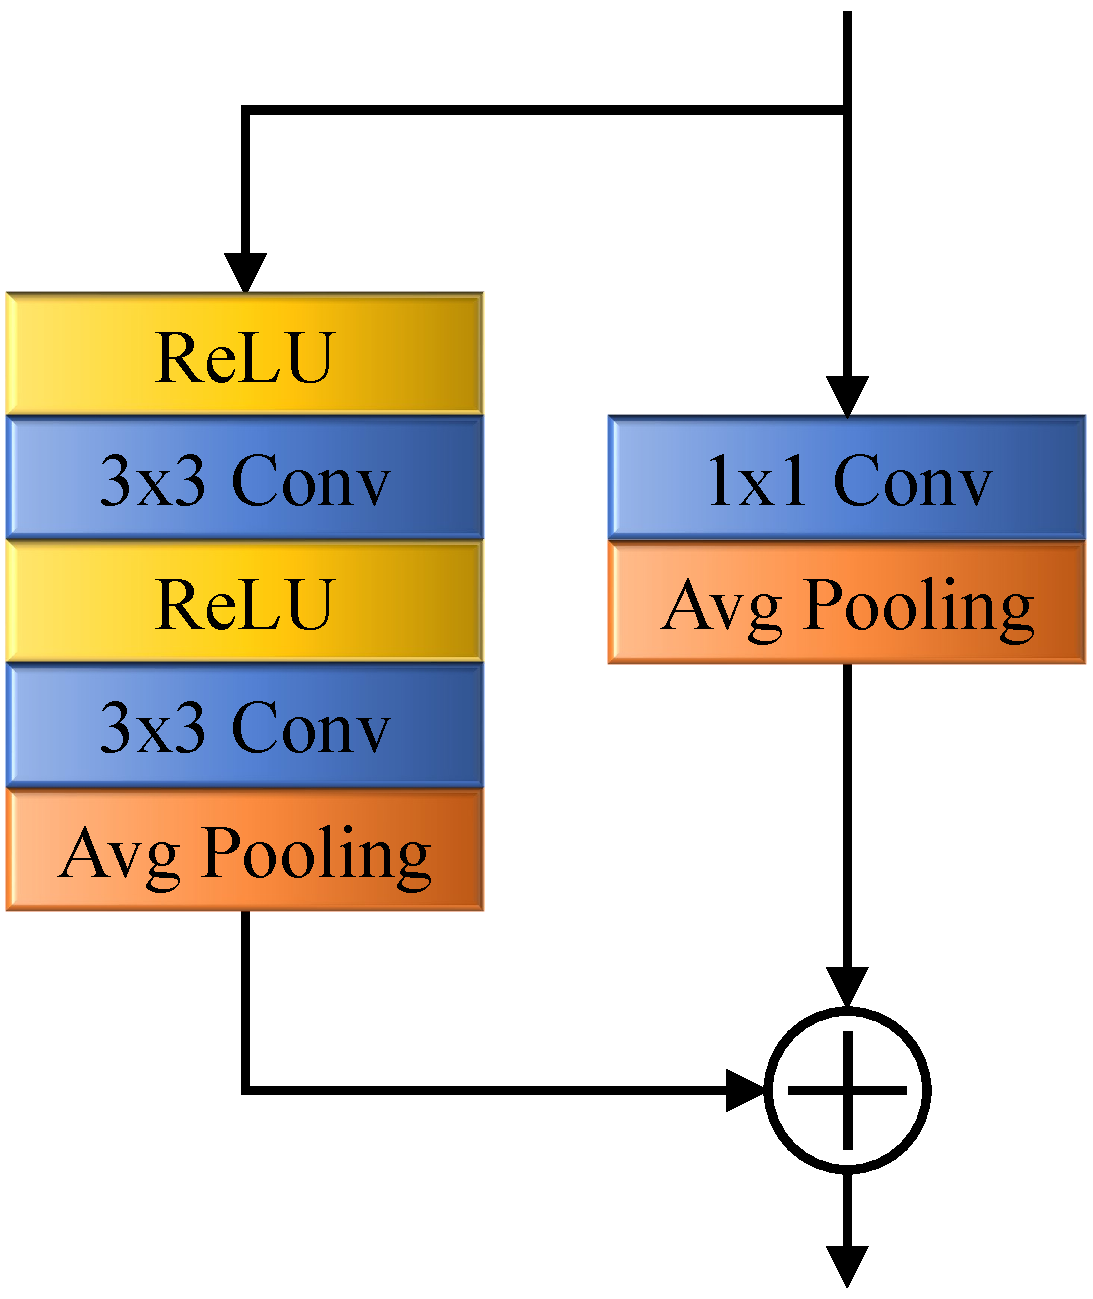
\includegraphics[width=0.6\columnwidth]{./biggan.pdf}
\caption{\textbf{A BigGAN's discriminator ResBlock}.}
\label{fig:BigGAN_ResBlock}
\end{figure}

To support this claim, in Fig.~\ref{tab:sparse_biggan}, we plot the histogram of norms of features for the pre-trained BigGAN critic \cite{brock2018large}, computed over $256$ randomly sampled $128\times 128$ images from the validation set within several residual blocks. In BigGAN, each ResBlock has two spatial convlutional layers (see Fig.~\ref{fig:BigGAN_ResBlock}). Interestingly, the inputs of the first convolutional layer in each ResBlock are not sparse, whereas the inputs of the second convolutional layer have some sparsity characteristics. This implies that the residual connection here eliminates sparsity. A possible solution could be to move the first ReLU so it would include the residual connection as commonly done in ResNets for image classification \cite{resnets}. Another possible solution may be to use a different compensation factor $g$ for different layers, according to their level of sparsity. We leave these for future work. Thus currently, our method is more applicable in feed-forward critic architectures, which actually dominate in image-to-image translation tasks.

\section{Additional Super-Resolution Results}
In Fig.~\ref{fig:sr} we show additional super-resolution results achieved with our approach, and compare them to the state-of-the-art ESRGAN.

\section{Experimental Setting}
In Tables \ref{tab:arch_gen_standard},\ref{tab:arch_resnet_cifar},\ref{tab:arch_resnet_stl},\ref{tab:arch_resnet_stargan} and \ref{tab:arch_sr}, we provide the exact network configuration for each of the experiments in the paper. In all implementations, we use cyclic padding for the convolutional layers of the critic. 

\newpage


\begin{figure*}[thp]
\centering
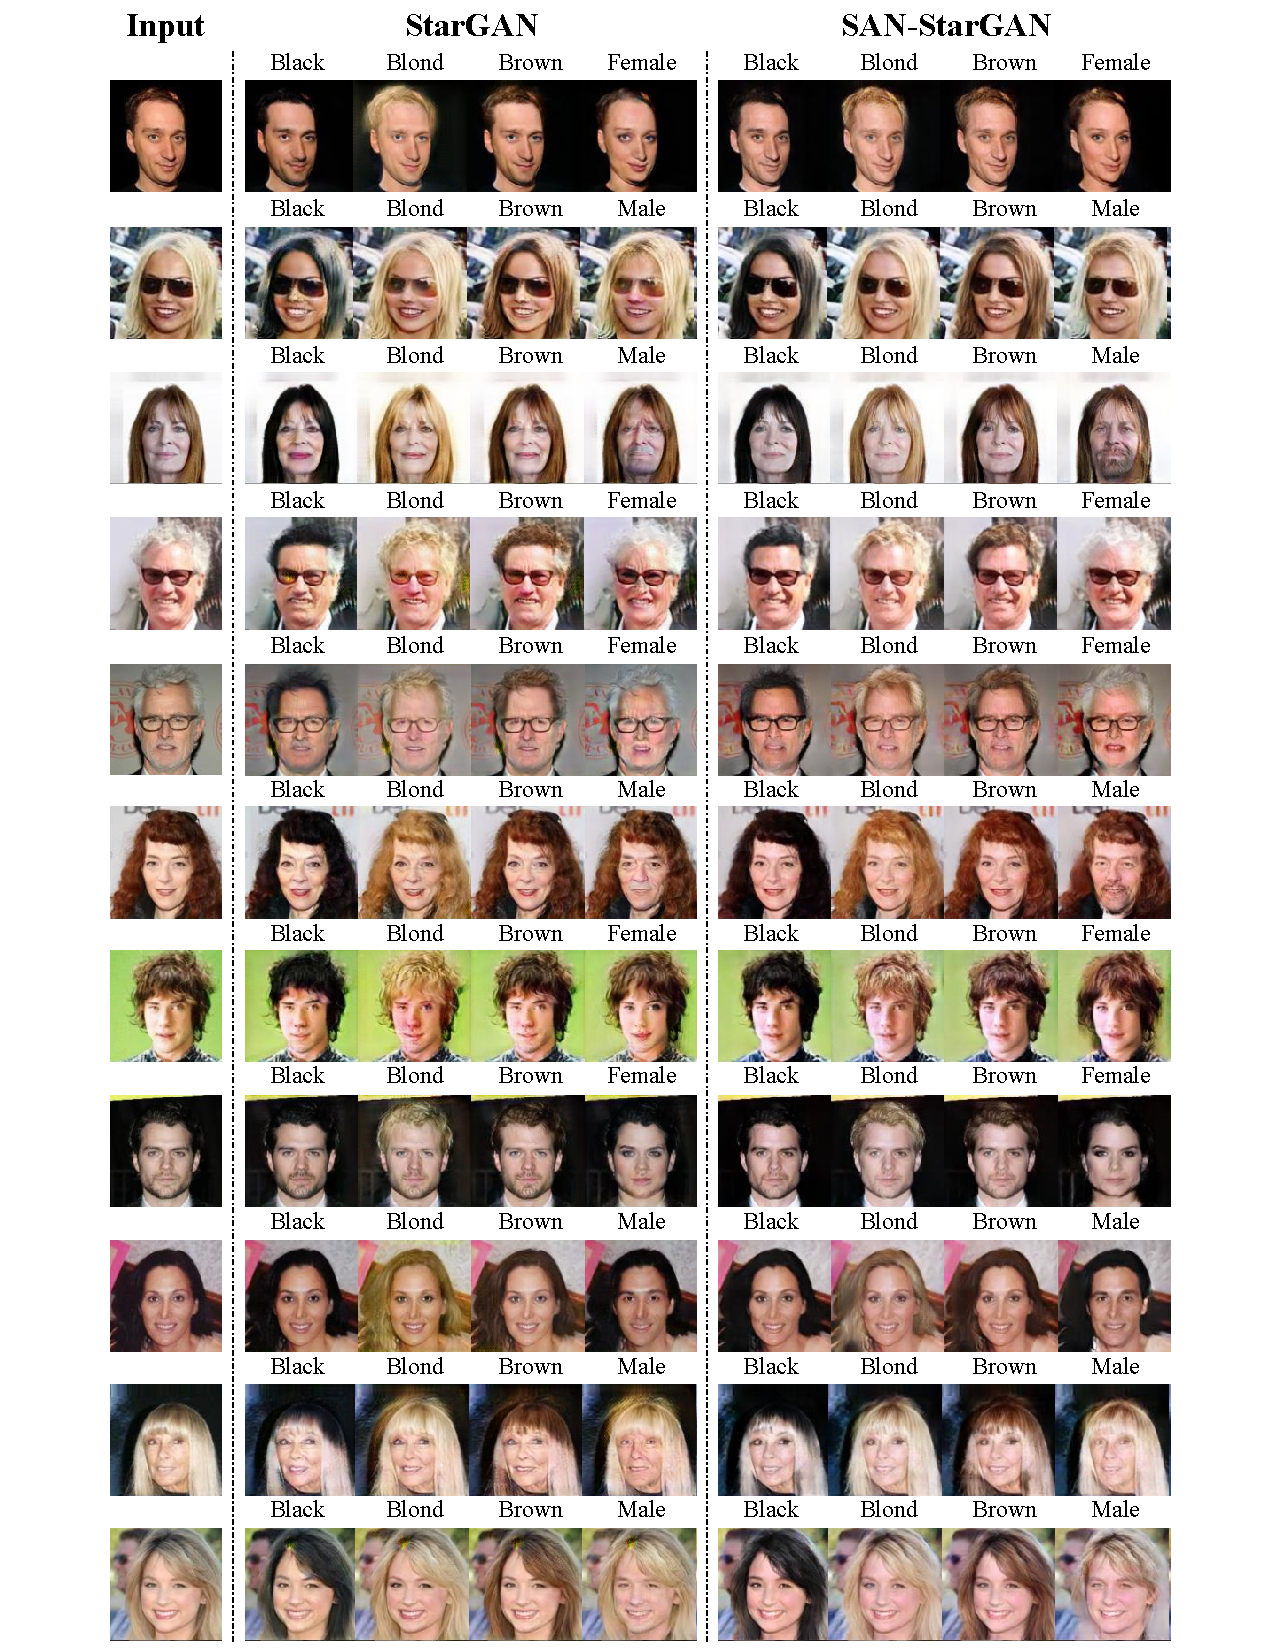
\includegraphics[width=0.825\textwidth]{./supplementary_v3.pdf}
\caption{\textbf{Visual comparison for image-to-image translation.} Each column corresponds to modifying a single attribute of the input image on the left. Our model manages to avoid artifacts (hallows around the head, colors on the face) and generate more photo-realistic images. Moreover, as opposed to the original StarGAN, our model does not modify attributes other than the desired one. For example, it does not add facial hair (as in row 1, column 1), fade sunglasses (as in row 2, columns 2,4), or change the apparent age (as in row 3, columns 1,2,3) when unnecessary.}
\label{fig:image2image_star}
\end{figure*}

\newpage

\begin{figure*}[thp]
\begin{center}
%\vspace{-3cm}
\begin{tabular}{ p{2.75cm} c c}
\vspace{-3.5cm}
$3rd$ Residual Block &
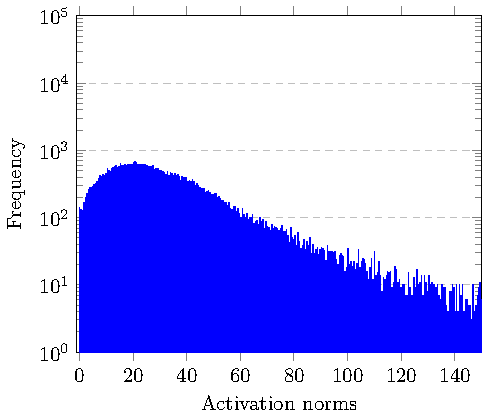
\includegraphics[scale=0.75]{./biggan_l4.pdf} &
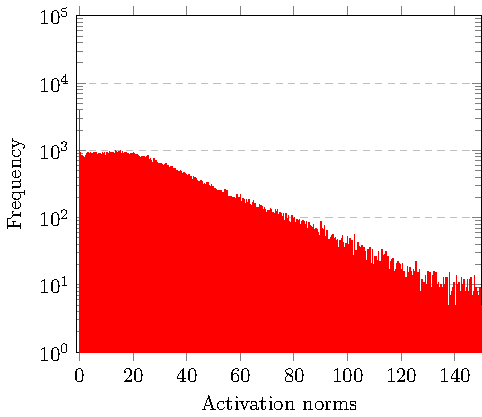
\includegraphics[scale=0.75]{./biggan_l5.pdf} \\

\vspace{-3.5cm}
$4th$ Residual Block &
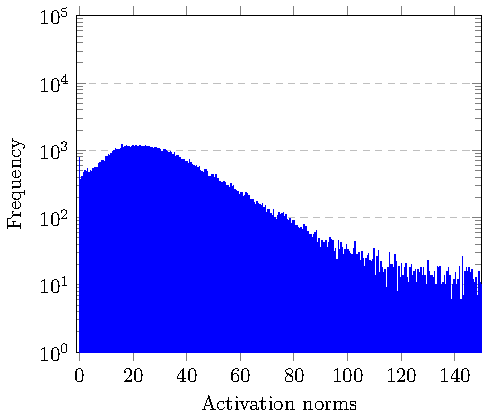
\includegraphics[scale=0.75]{./biggan_l6.pdf} &
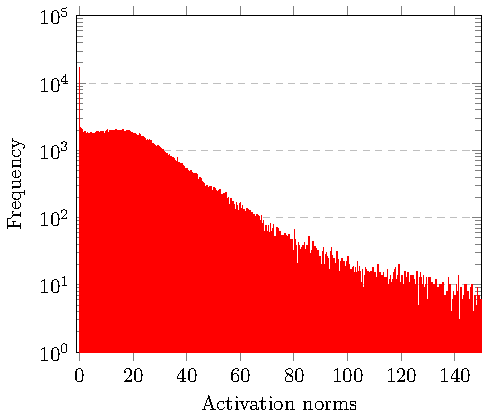
\includegraphics[scale=0.75]{./biggan_l7.pdf} \\

\vspace{-3.5cm}
$5th$ Residual Block &
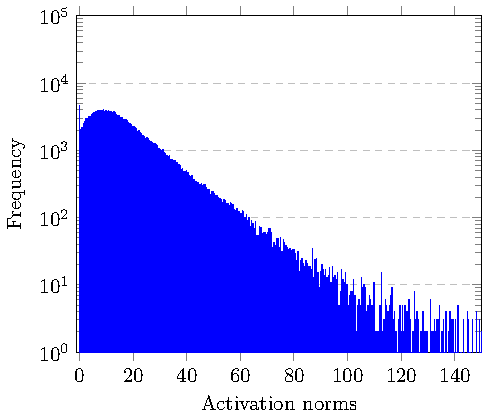
\includegraphics[scale=0.75]{./biggan_l8.pdf} &
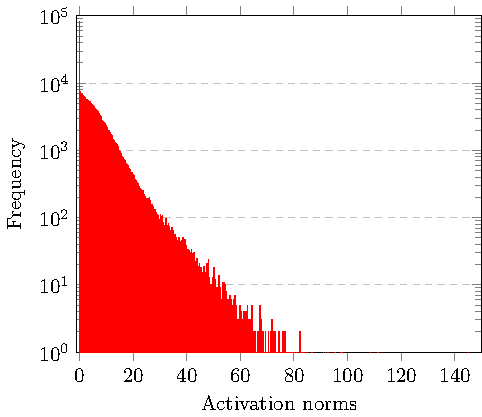
\includegraphics[scale=0.75]{./biggan_l9.pdf} \\ \\
&
\hspace{1cm}
1st Convolution &
\hspace{1cm}
2nd Convolution

\end{tabular}
\caption{\textbf{Channel sparsity in BigGAN.} The histograms of the channel norms for several convolutional layers in a pre-trained BigGAN critic network, computed over $256$ randomly chosen samples from the ImageNet training set. The inputs to the first convolution (blue) are less sparse than the inputs to the second convolution (red). Note particularly the sharp peak at 0 in the red histograms.}
\label{tab:sparse_biggan}
\end{center}
\end{figure*}

\newpage

\begin{figure*}[thp]
	\centering
	\vspace{-0.5cm}
	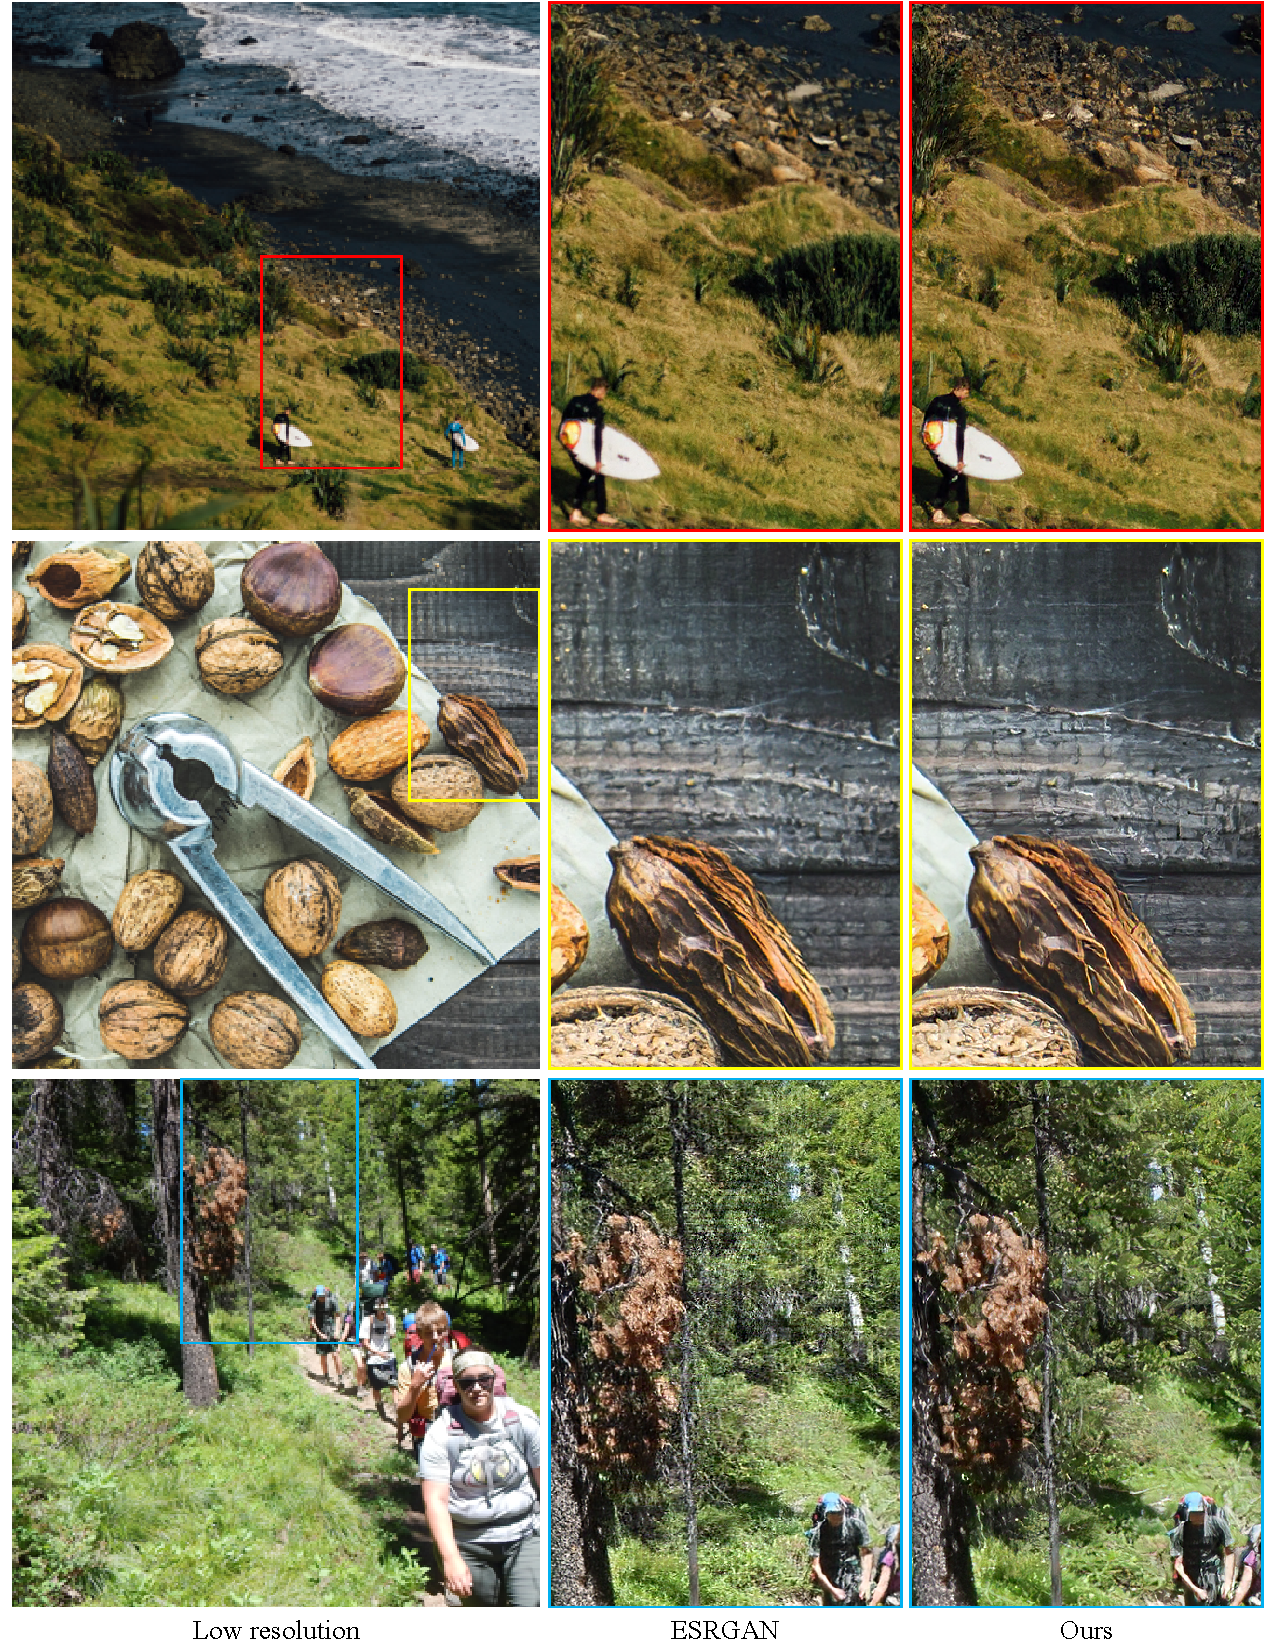
\includegraphics[width=0.95\textwidth]{./figure_v2.pdf}
	\vspace{-0.2cm}
	\caption{\textbf{Additional super-resolution comparisons.}}
	\label{fig:sr}
\end{figure*}

\newpage

\begin{table*}[thp]
	\begin{center}
		\begin{tabular}{ c  c }
			Generator & Critic \\  
			\begin{tabular}{ c }
				\hline \hline
				\\
				$z \in \mathbb{R}^{128} \sim \mathit{N}(0,I)$ \\
				dense $\Rightarrow M_g \times M_g \times 512$\\
				$3\times 3$, stride=2 deconv. BN 256 ReLU\\
				$3\times 3$, stride=2 deconv. BN 128 ReLU\\
				$3\times 3$, stride=2 deconv. BN 64 ReLU\\
				$3\times 3$, stride=1 conv. 3 Tanh\\ 
				\\ \\ \\
			\end{tabular} &  
			\begin{tabular}{ c } 
				\hline \hline
				\\
				RGB image $x \in \mathbb{R}^{M\times M \times 3}$\\
				$3\times 3$, stride=1 conv. 64 lReLU\\
				$3\times 3$, stride=2 conv. 64 lReLU\\
				$3\times 3$, stride=1 conv. 128 lReLU\\
				$3\times 3$, stride=2 conv. 128 lReLU\\
				$3\times 3$, stride=1 conv. 256 lReLU\\
				$3\times 3$, stride=2 conv. 256 lReLU\\
				$3\times 3$, stride=1 conv. 512 lReLU\\
				dense $\Rightarrow 1$\\
			\end{tabular}
			\\ & \\
		\end{tabular}
		\caption{\textbf{The standard architecture used for image generation.} We use a standard CNN model for our unconditional image generation experiments on CIFAR-10 and STL-10. The slopes of all leaky-ReLU (lReLU) functions are set to $0.1$. For the generator, we use  $M_g=4$ for CIFAR-10 and $M_g=6$ for STL-10. For the critic, we use $M=32$ for CIFAR-10 and $M=48$ for STL-10.}
		\label{tab:arch_gen_standard}
	\end{center}
\end{table*}


\begin{table*}[thp]
	\begin{center}
		\begin{tabular}{ c  c }
			Generator & Critic \\  
			\begin{tabular}{ c }
				\hline \hline
				\\
				$z \in \mathbb{R}^{128} \sim \mathit{N}(0,I)$ \\
				dense $\Rightarrow 4 \times 4 \times 256$\\
				ResBlock, up-sample, 256\\
				ResBlock, up-sample, 256\\
				ResBlock, up-sample, 256\\
				BN, ReLU, $3\times 3$ conv., 3 Tanh\\ 
				\\ \\
			\end{tabular} &  
			\begin{tabular}{ c } 
				\hline \hline
				\\
				RGB image $x \in \mathbb{R}^{32\times 32 \times 3}$\\
				ResBlock, down-sample, 128\\
				ResBlock, down-sample, 128\\
				ResBlock, 128\\
				ResBlock, 128\\
				ReLU\\
				Global avg. pooling\\
				dense $\Rightarrow 1$\\
			\end{tabular}
			\\ & \\
		\end{tabular}
		\caption{\textbf{The ResNet architecture used for image generation on CIFAR-10.} The ResBlock comprises a sequences of batch-norm, ReLU, convolution, batch-norm, ReLU and convolution layers. In the critic, batch-norm layers are removed from the ResBlock.}
		\label{tab:arch_resnet_cifar}
	\end{center}
\end{table*}


\begin{table*}[thp]
	\begin{center}
		\begin{tabular}{ c  c }
			Generator & Critic \\  
			\begin{tabular}{ c }
				\hline \hline
				\\
				$z \in \mathbb{R}^{128} \sim \mathit{N}(0,I)$ \\
				dense $\Rightarrow 6 \times 6 \times 512$\\
				ResBlock, up-sample, 256\\
				ResBlock, up-sample, 128\\
				ResBlock, up-sample, 64\\
				BN, ReLU, $3\times 3$ conv., 3 Tanh\\ 
				\\ \\
			\end{tabular} &  
			\begin{tabular}{ c } 
				\hline \hline
				\\
				RGB image $x \in \mathbb{R}^{48\times 48 \times 3}$\\
				ResBlock, down-sample, 64\\
				ResBlock, down-sample, 128\\
				ResBlock, down-sample, 256\\
				ResBlock, down-sample, 512\\
				ReLU\\
				Global avg. pooling\\
				dense $\Rightarrow 1$\\
			\end{tabular}
			\\ & \\
		\end{tabular}
		\caption{\textbf{The ResNet architecture used for image generation on STL-10.} The ResBlock comprises a sequences of batch-norm, ReLU, convolution, batch-norm, ReLU and convolution layers. In the critic, batch-norm layers are removed from the ResBlock. In comparison to \cite{spectral}, we remove the discriminator's last ResBlock.}
		\label{tab:arch_resnet_stl}
	\end{center}
\end{table*}


\begin{table*}[thp]
	\begin{center}
		\begin{tabular}{ c  c }
			Generator & Critic \\  
			\begin{tabular}{ c }
				\hline \hline
				\\
				RGB image $x \in \mathbb{R}^{128\times 128 \times 3}$\\
				$7\times 7$, stride=1 conv. IN 64 ReLU\\
				$4\times 4$, stride=2 conv. IN 128 ReLU\\
				$4\times 4$, stride=2 conv. IN 256 ReLU\\
				ResBlock, 256\\
				ResBlock, 256\\
				ResBlock, 256\\
				ResBlock, 256\\
				ResBlock, 256\\
				ResBlock, 256\\
				$4\times 4$, stride=2 deconv. IN 128 ReLU\\
				$4\times 4$, stride=2 deconv. IN 64 ReLU\\
				$7\times 7$ conv., 3 Tanh\\ 
			\end{tabular} &  
			\begin{tabular}{ c } 
				\hline \hline
				\\
				RGB image $x \in \mathbb{R}^{128\times 128 \times 3}$\\
				$3\times 3$, stride=2 conv. 64 lReLU\\
				$3\times 3$, stride=2 conv. 128 lReLU\\
				$3\times 3$, stride=2 conv. 256 lReLU\\
				$3\times 3$, stride=2 conv. 512 lReLU\\
				$3\times 3$, stride=2 conv. 1024 lReLU\\
				$3\times 3$, stride=2 conv. 2048 lReLU\\
				$3\times 3$, conv. 1 | $2\times 2$, conv. $n_d$\\
				\\ \\ \\ \\ \\
			\end{tabular}
			\\ & \\
		\end{tabular}
		\caption{\textbf{Image-to-image translation architectures.} For the generator, we perform instance normalization (IN) in all layers except the last output layer. The ResBlock comprises a sequences of convolution, instance-norm, ReLU, convolution and instance-norm layers. In the critic, we use leaky ReLU with slope $0.01$. Here, $n_d$ represents the number of domains, as the critic outputs a 1-hot classification vector of length $n_d$.}
		\label{tab:arch_resnet_stargan}
	\end{center}
\end{table*}


\begin{table*}[thp]
	\begin{center}
		\begin{tabular}{ c  c }
			Generator & Critic \\  
			\begin{tabular}{ c }
				\hline \hline
				\\
				RGB image $x \in \mathbb{R}^{\frac{N}{4}\times \frac{N}{4} \times 3}$\\
				$3\times 3$, stride=1 conv. 64 lReLU\\
				ResBlock, 64\\
				ResBlock, 64\\
				$\vdots$ \\
				ResBlock, 64\\
				$3\times 3$, stride=1 conv. 256, PS, lReLU\\
				$3\times 3$, stride=1 conv. 256, PS, lReLU\\
				$3\times 3$, stride=1 conv. 64, lReLU\\
				$3\times 3$, stride=1 conv. 3, +up-sample(x)\\
			\end{tabular} &  
			\begin{tabular}{ c } 
				\hline \hline
				\\
				RGB image $x \in \mathbb{R}^{128\times 128 \times 3}$\\
				$3\times 3$, stride=1 conv. 64 lReLU\\
				$3\times 3$, stride=2 conv. 64 lReLU\\
				$3\times 3$, stride=1 conv. 128 lReLU\\
				$3\times 3$, stride=2 conv. 128 lReLU\\
				$3\times 3$, stride=1 conv. 256 lReLU\\
				$3\times 3$, stride=2 conv. 256 lReLU\\
				$3\times 3$, stride=1 conv. 512 lReLU\\
				$3\times 3$, stride=2 conv. 512 lReLU\\
				dense $\Rightarrow 100$, lReLU\\
				dense $\Rightarrow 1$\\
			\end{tabular}
			\\ & \\
		\end{tabular}
		\caption{\textbf{Single image super-resolution architectures.} We use leaky ReLU with slope $0.1$, and pixelshuffle (PS) for the up-sampling operation. The ResBlock comprises a sequences of convolution, ReLU, and convolution layers. The generator consists of $16$ residual blocks as in \cite{srgan}.}
		\label{tab:arch_sr}
	\end{center}
\end{table*}

